\chapter{\ChapterTitleScope}
\label{sec:zakres-funkcjonalnosci}


\section{Kontekst użytkowania aplikacji}

Głównym zadaniem aplikacji jest oferowanie możliwości
rozgrywania gry w~brydża. Strona internetowa aplikacji ma być
przystosowana do dowolnego rozmiaru ekranu urządzenia, z~którego mógłby
korzystać użytkownik. Dzięki temu można skorzystać z~aplikacji, wykorzystując
telefon, komputer stacjonarny, laptop lub nawet telewizor. Wymagany
jest tylko dostęp do Internetu.
Schematy interakcji użytkownika z~aplikacją zostały przedstawione na rysunkach
\ref{fig:figma_userflow} i~\ref{fig:figma_gameflow}. \\

\begin{figure}[h!]
  \centering
  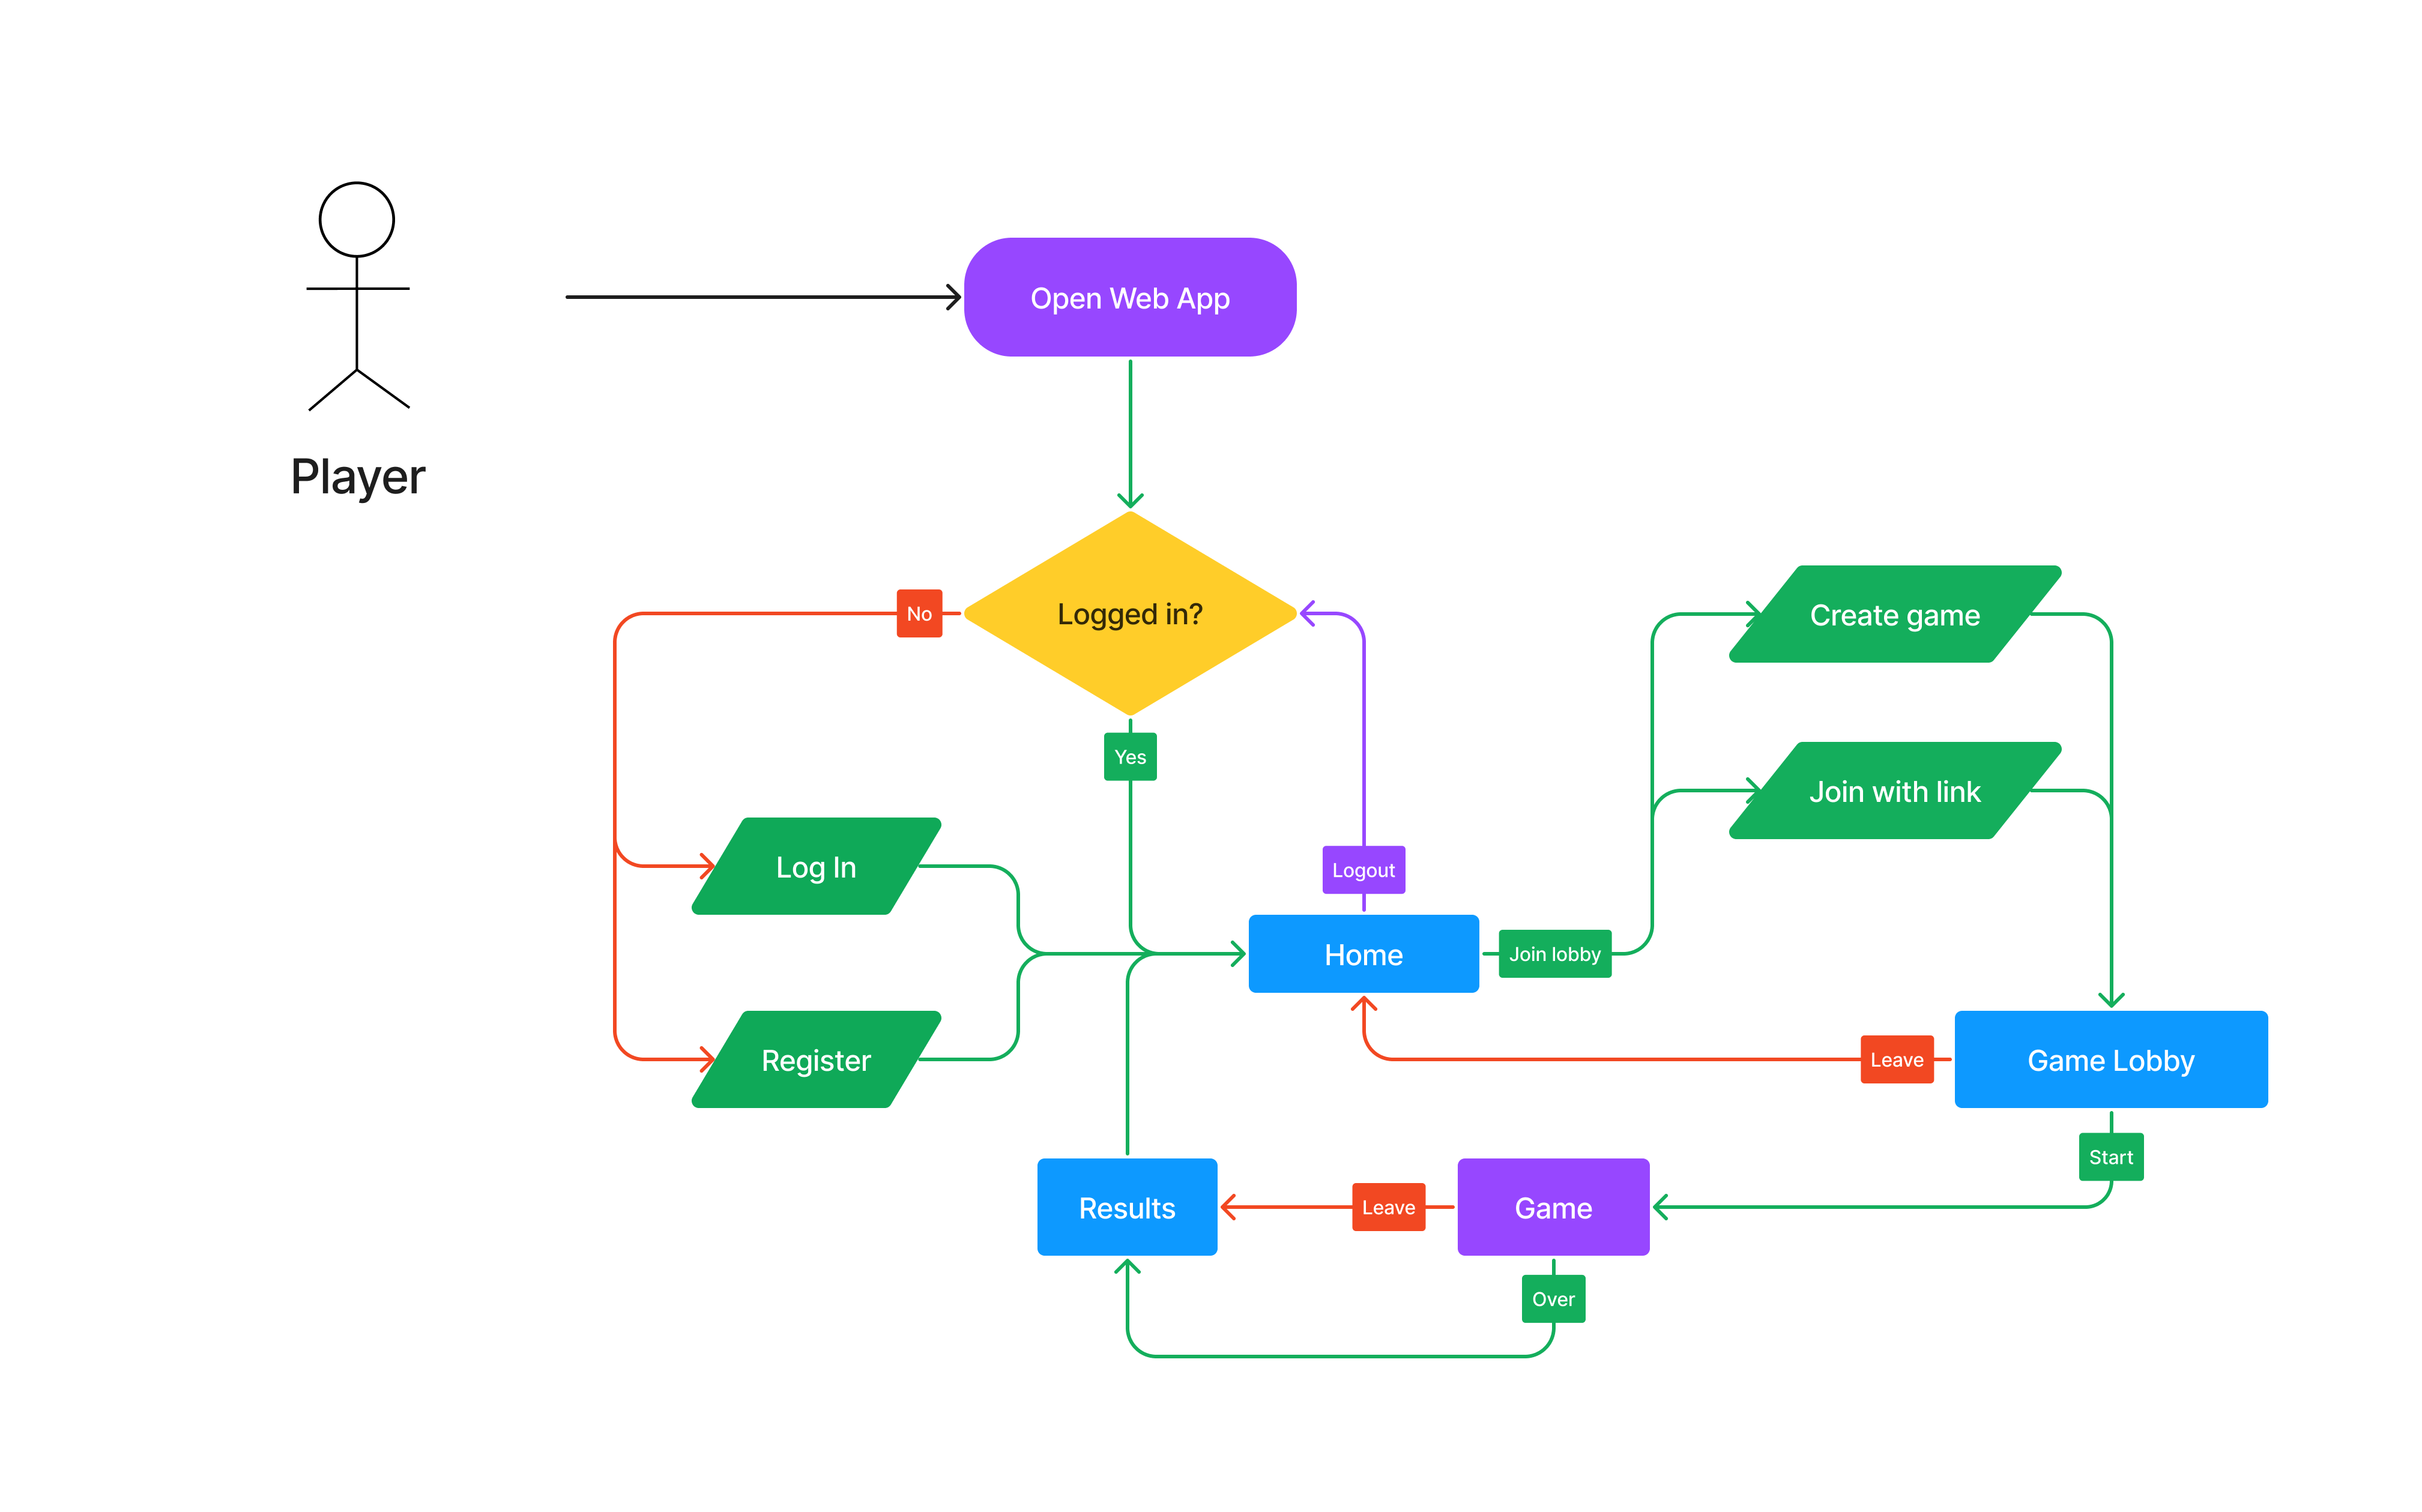
\includegraphics[width=0.9\textwidth]{img/flow-aplikacji/user_flow.png}
  \caption{Schemat interakcji użytkownika z aplikacją}
  \label{fig:figma_userflow}
\end{figure}

\begin{figure}[h!]
  \centering
  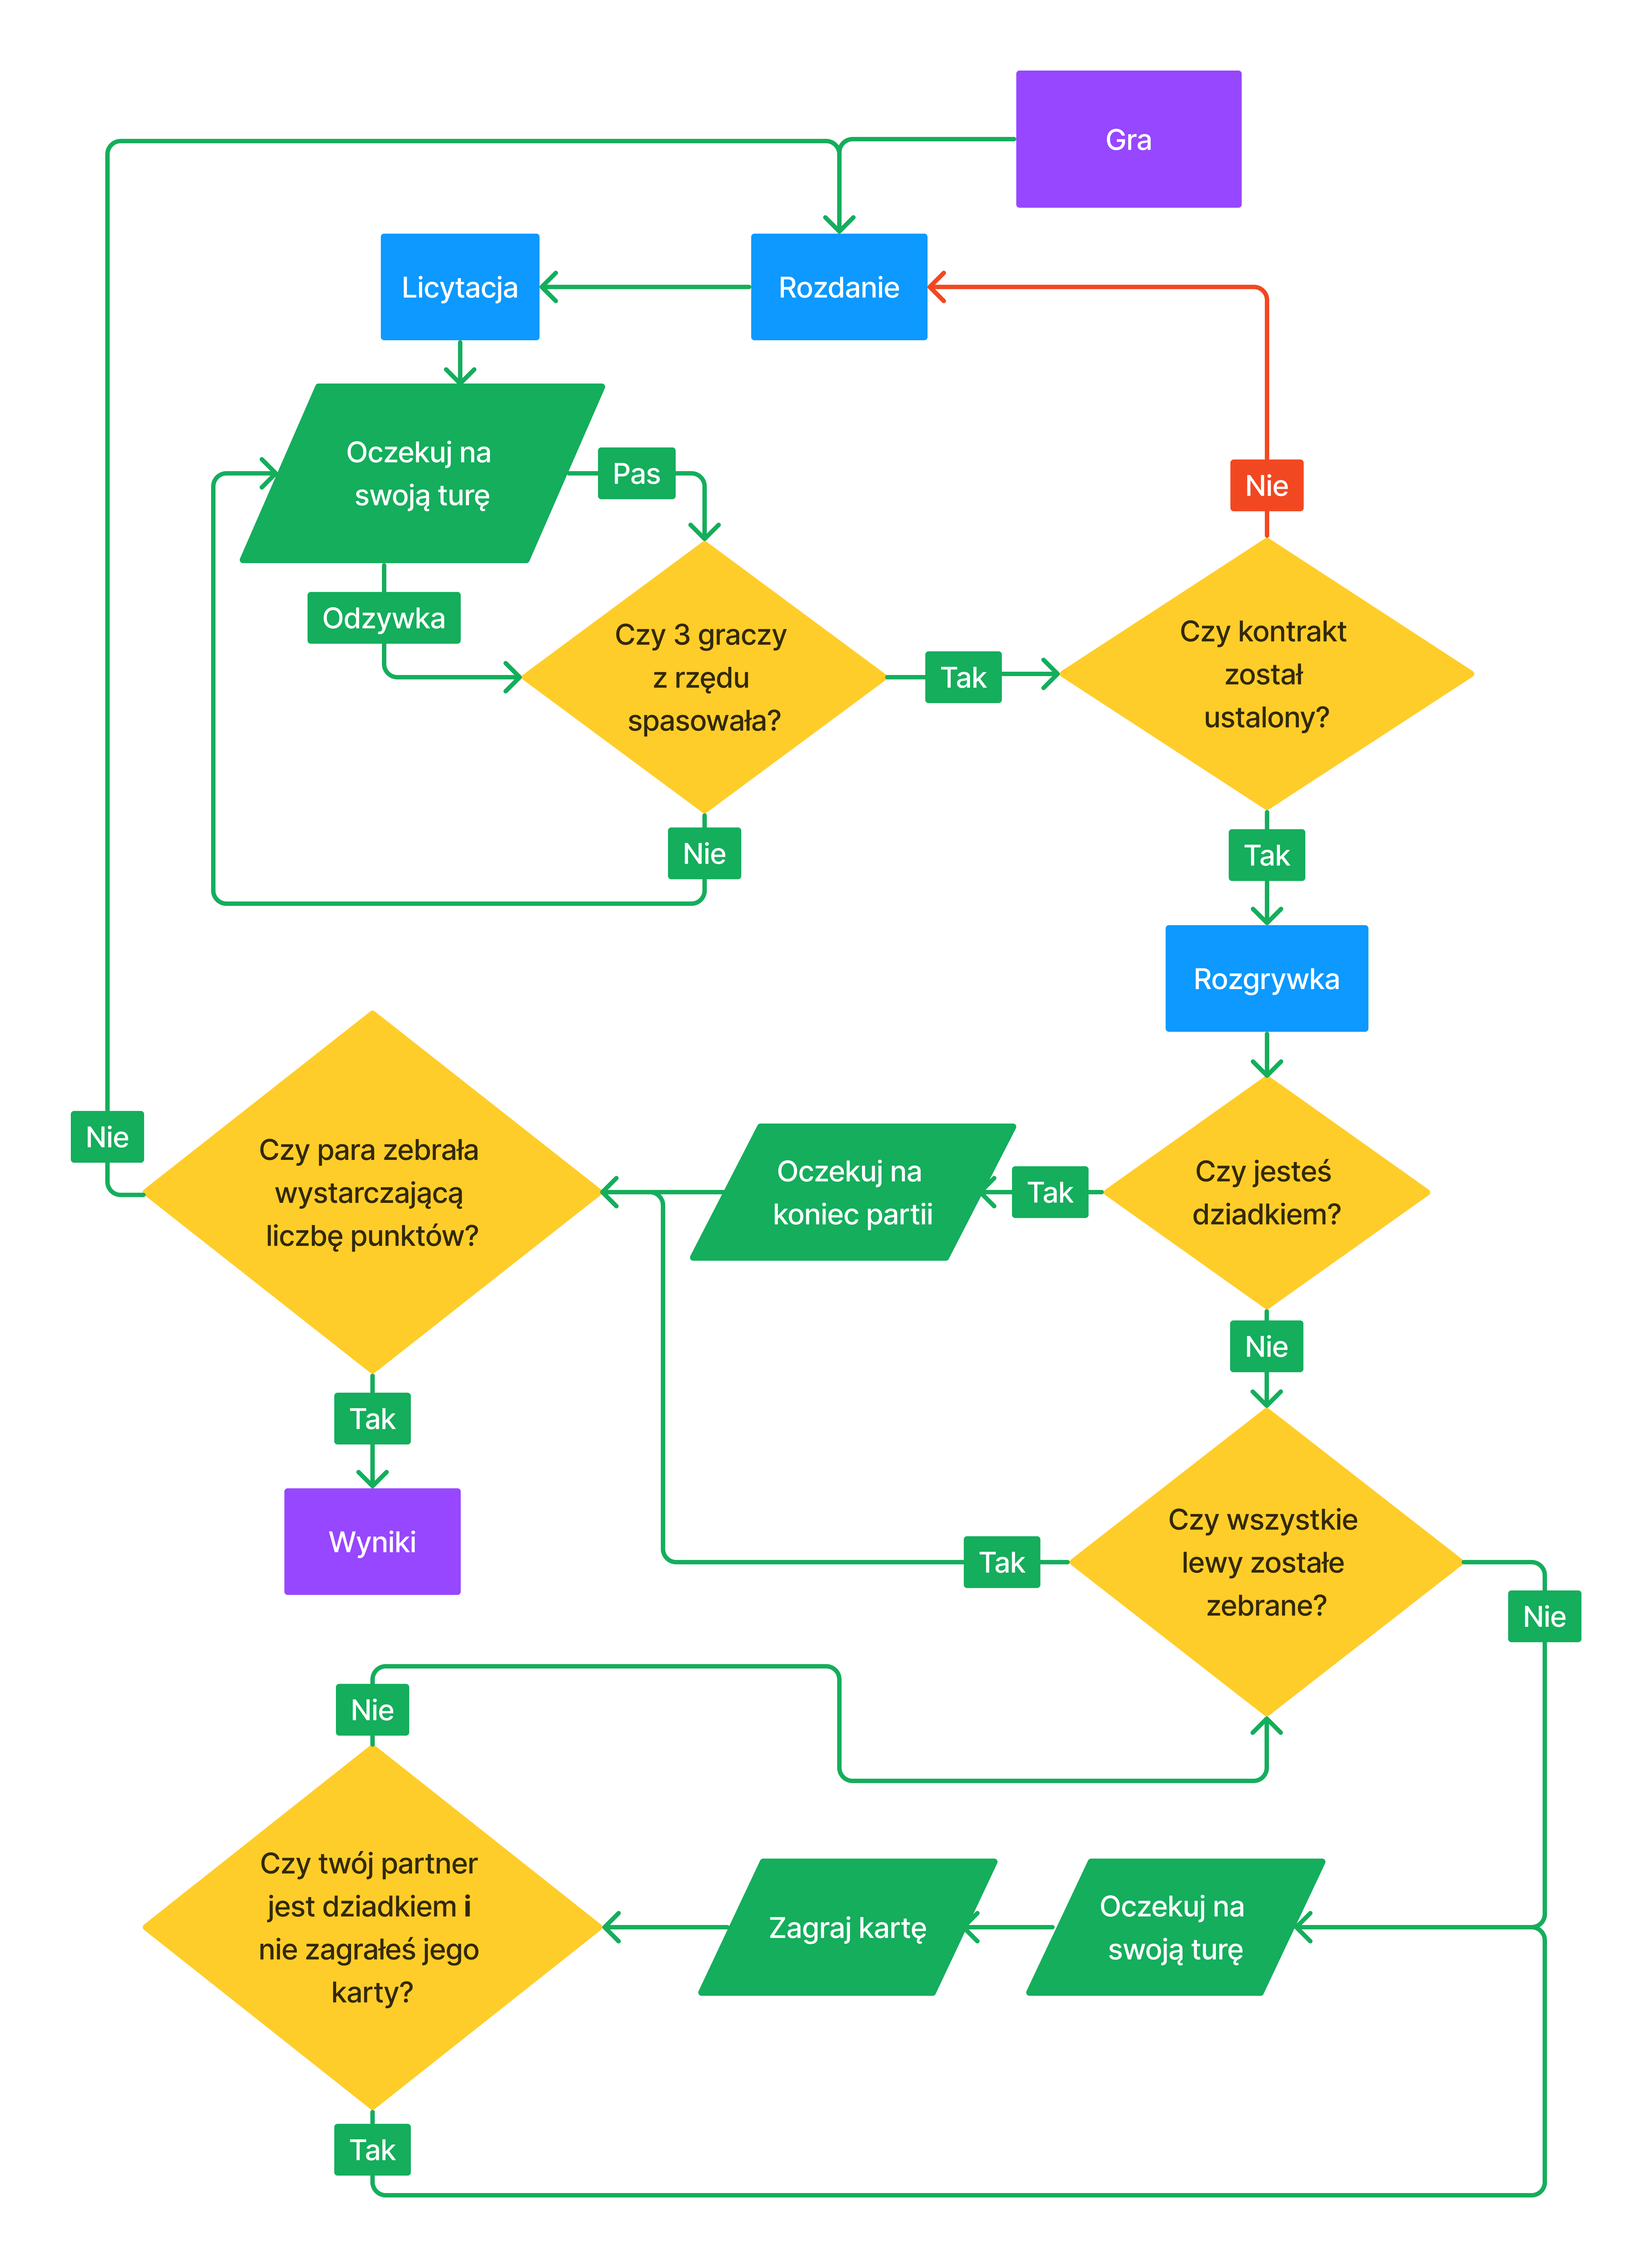
\includegraphics[width=\textwidth]{img/flow-aplikacji/game_flow.png}
  \caption{Schemat interakcji użytkownika z aplikacją podczas rozgrywki brydża}
  \label{fig:figma_gameflow}
\end{figure}

\newpage

W~systemie aplikacji zdefiniowane są dwa typy użytkowników:
\begin{itemize}
  \item \textbf{anonimowy użytkownik} -- osoba niezalogowana, która nie
        posiada dostępu do funkcjonalności aplikacji związanych
        z~rozgrywką.

  \item \textbf{zalogowany użytkownik} -- zalogowana osoba posiadająca konto
        w~aplikacji, mająca pełny dostęp do jej funkcjonalności.
\end{itemize}

Funkcjonalności dostępne dla poszczególnych użytkowników:
\begin{itemize}
  \item \textbf{anonimowy użytkownik}:
        \begin{itemize}
          \item rejestracja nowego konta w~systemie aplikacji.
          \item logowanie do konta utworzonego w~systemie aplikacji.
        \end{itemize}

  \item \textbf{zalogowany użytkownik}:
        \begin{itemize}
          \item wylogowanie z~konta (przejście w~stan użytkownika anonimowego),
          \item tworzenie i~dołączanie do rozgrywek w brydża --
                gdy użytkownik założy lub zostanie jedynym
                użytkownikiem lobby, to staje się jego
                hostem,
          \item zarządzanie lobby -- może decydować o~graczach znajdujących się wraz
                z~nim w~lobby; może decydować o~ich pozycji lub ich wyrzucić
                ze wspólnej sesji\footnote{Sesja oznacza to samo co lobby, czyli
                  abstrakcję łączącą wielu graczy w~obrębie jednej
                  rozgrywki};
                może uzupełnić wolne miejsca wirtualnym asystentem
                z~określeniem jego poziomu trudności.
        \end{itemize}
\end{itemize}

\FloatBarrier

\section{Przypadki użycia}

\subsection{Rejestracja i logowanie do aplikacji}

Aby uzyskać dostęp do większości funkcjonalności aplikacji, wymagane
jest posiadanie konta. Anonimowy użytkownik może je utworzyć, klikając
opcję "Register"\xspace w~nagłówku strony. Po kliknięciu użytkownik
zostanie przekierowany do formularza rejestracyjnego.
Do utworzenia konta wymagane jest podanie własnego
pseudonimu, adresu e-mail oraz hasła. Aby uzyskać dostęp do utworzonego
konta, należy kliknąć "Log in"\xspace w~nagłówku strony, po czym
w~formularzu podać dane wykorzystanie podczas rejestracji (Rys.~\ref{fig:figma_xd_login}).

\begin{figure}[hbt!]
  \centering
  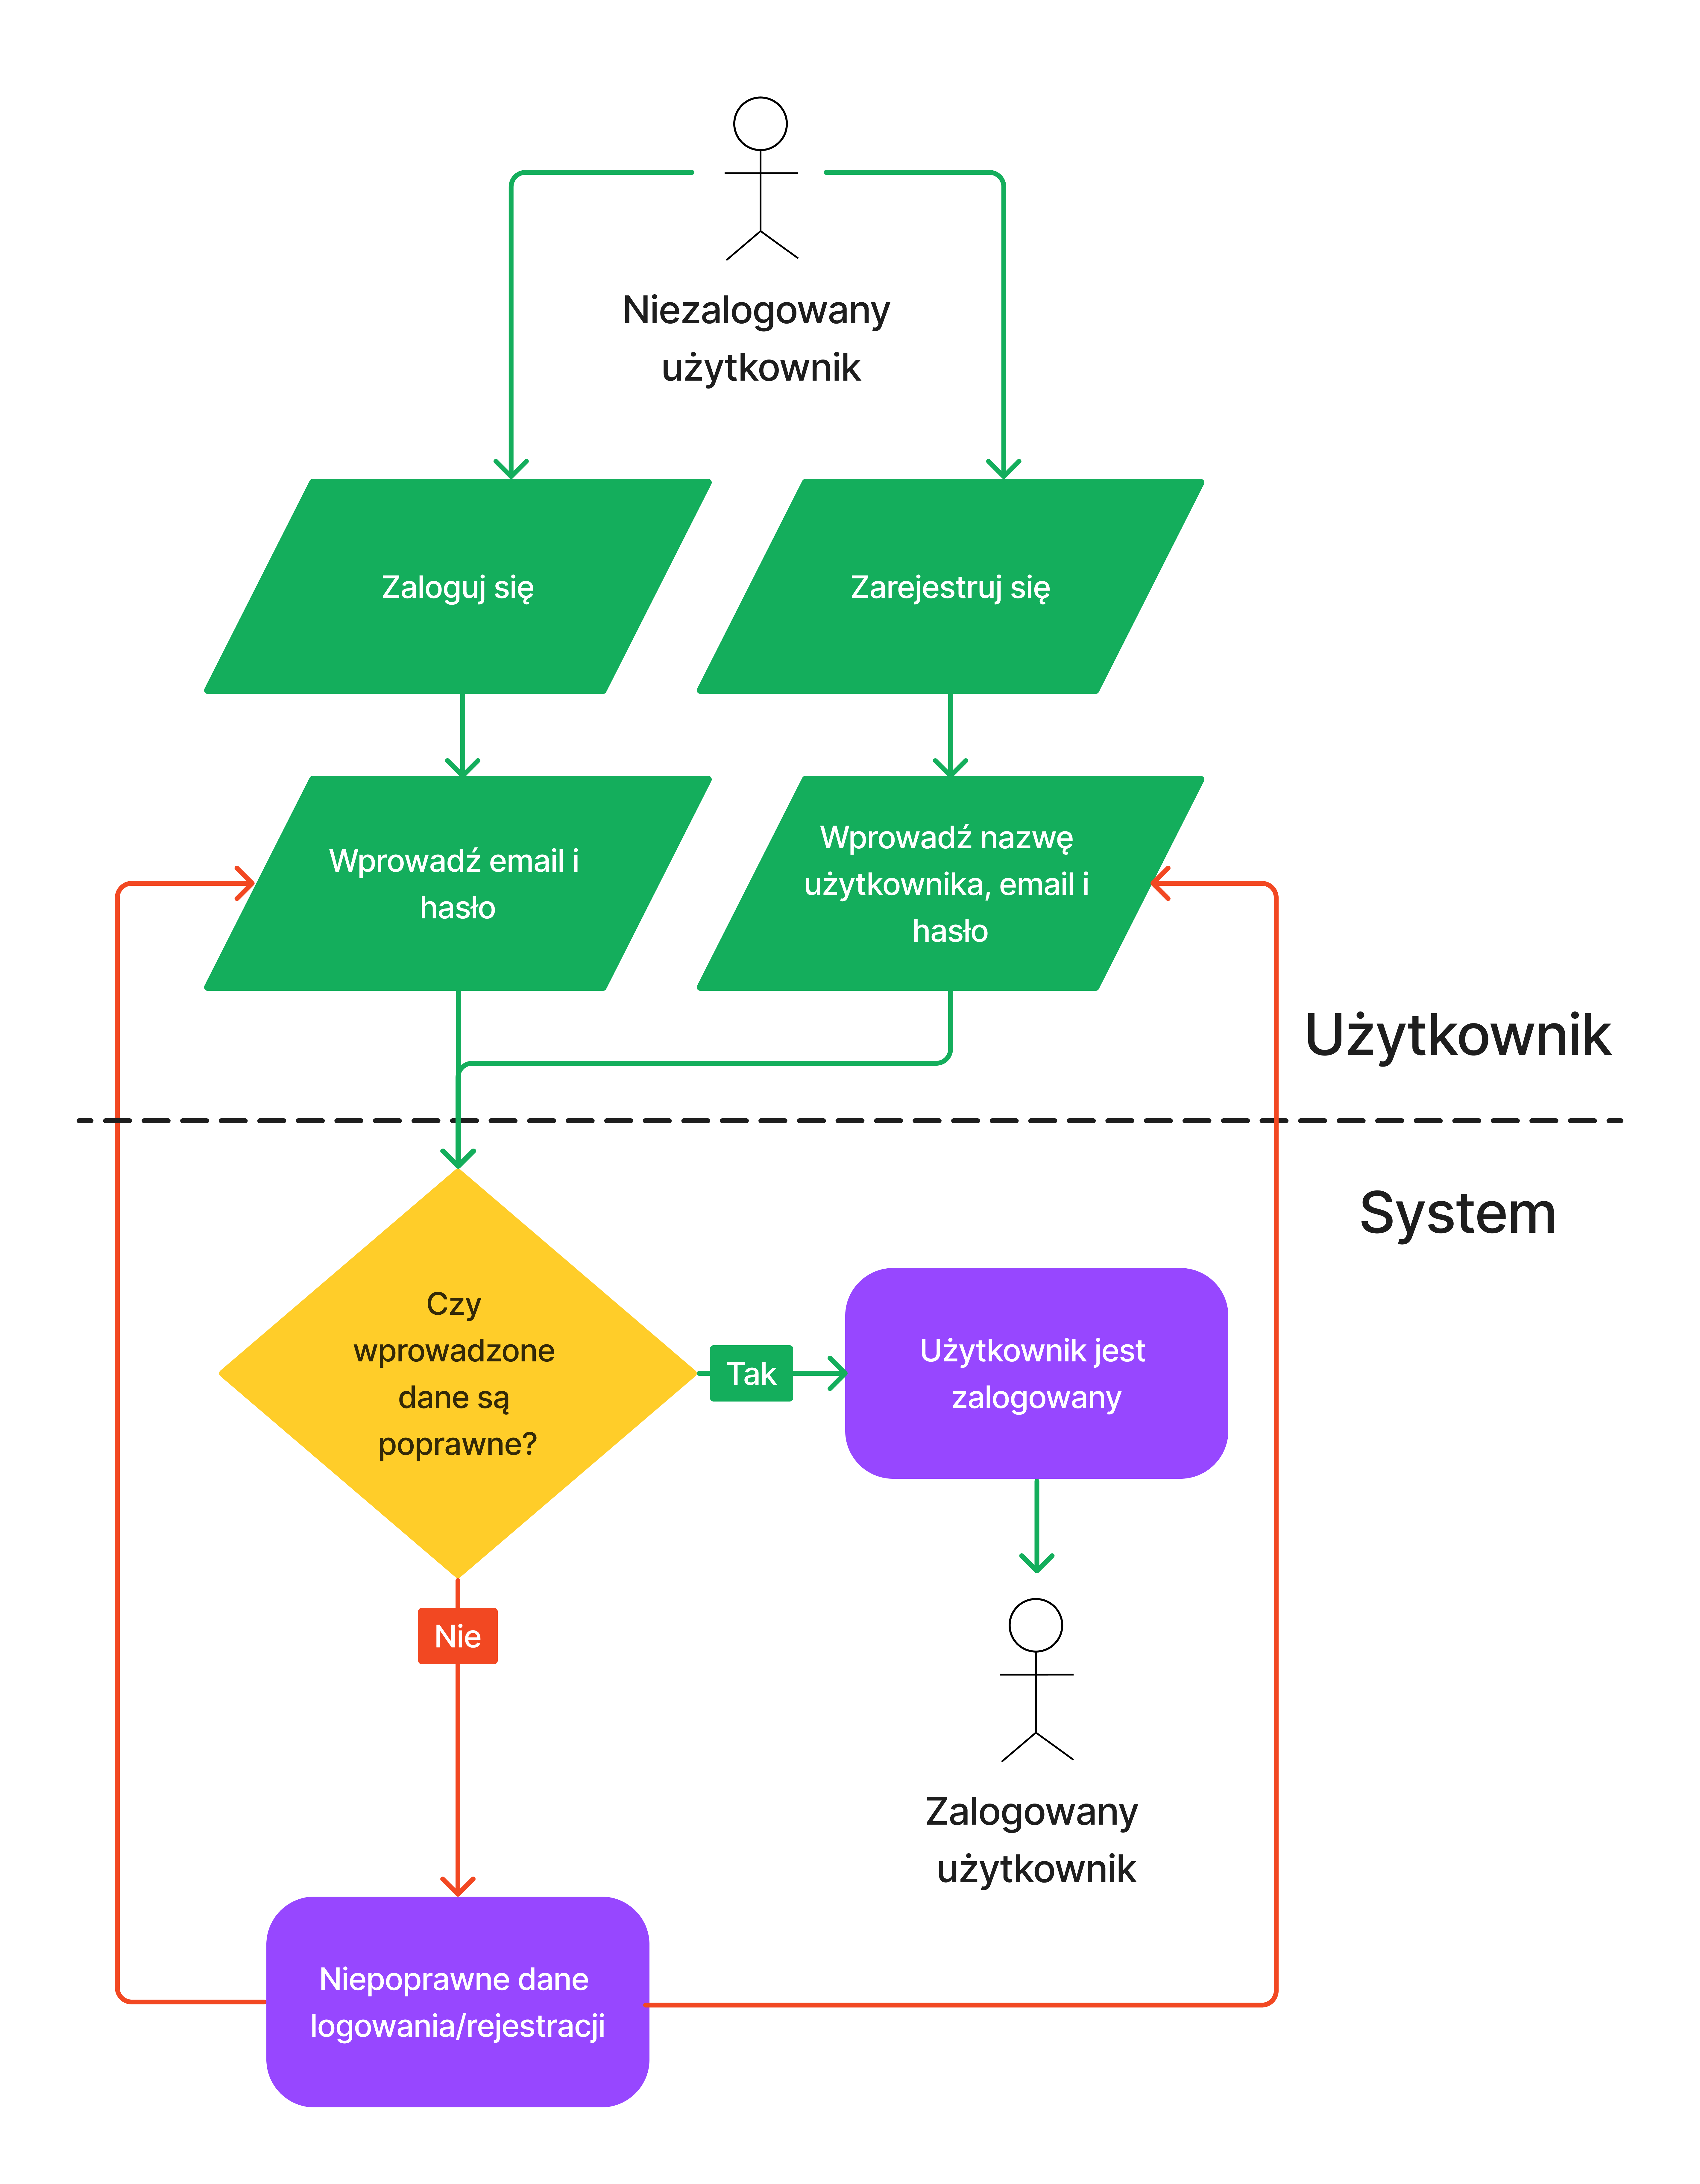
\includegraphics[width=0.9\textwidth]{img/schematy/login.png}
  \caption{Schemat logowania i~rejestracji użytkownika}
  \label{fig:figma_xd_login}
\end{figure}

W~przypadku nieprawidłowo podanych danych podczas rejestracji
lub logowania, wystąpienia błędów wynikających z~połączenia internetowego lub
niedostępnego serwerem autentykacji, użytkownik otrzyma odpowiednią
informację na ekranie.

\FloatBarrier


\subsection{Lobby}

\subsubsection{Tworzenie lobby}

Rozpoczęcie gry w~brydża jest dostępne z~poziomu lobby. Aby utworzyć
lobby, należy kliknąć "Create lobby"\xspace na głównym panelu
aplikacji. Przekieruje ono użytkownika do nowego lobby, którego staje
się hostem. Do utworzonego lobby zostanie wygenerowany
unikalny identyfikator, zwany dalej kodem. Użytkownik będzie mógł go skopiować
i~udostępnić, np. znajomym, aby mogli oni do niego dołączyć (Rys.~\ref{fig:figma_xd_create_join_lobby}).


\subsubsection{Dołączanie do lobby}

Gdy użytkownik otrzyma kod do lobby od innego użytkownika, może
do niego dołączyć, poprzez główny panel aplikacji. Należy wkleić
kod w~odpowiednie pole i~klikając opcję "Join"\xspace
dołączyć do przypisanego do kodu lobby (Rys.~\ref{fig:figma_xd_create_join_lobby}).

\begin{figure}[hbt!]
  \centering
  \includegraphics[width=0.9\textwidth]{img/schematy/create_join_lobby.png}
  \caption{Schemat tworzenia i dołączania do lobby}
  \label{fig:figma_xd_create_join_lobby}
\end{figure}

\FloatBarrier


\subsubsection{Zarządzanie lobby}

Jeżeli użytkownik jest hostem lub został jedynym
użytkownikiem w~lobby, może on zarządzać stanem innych graczy (Rys.~\ref{fig:figma_xd_manage_lobby}).
Posiada on następujące możliwości:
\begin{itemize}
  \item zamiana pozycji w lobby -- dwie wybrane pozycje są zamieniane miejscami
        (może być to gracz lub puste miejsce),
  \item usunięcie gracza z lobby -- gracz opuszcza lobby i~nie będzie
        mógł już ponownie do niego dołączyć,
  \item awans użytkownika na hosta lobby -- wybrany gracz, będący użytkownikiem
        aplikacji, otrzymuje uprawnienia hosta; poprzedni host traci uprawnienia hosta,
  \item zajęcie wolnej pozycji jako wirtualny asystent -- wybrana pozycja
        w~grze będzie kontrolowana przez asystenta
        i~uczestniczyć w~rozgrywce jako partner lub przeciwnik,
  \item zamknięcie lobby -- jeżeli host jest ostatnim
        użytkownikiem w~lobby, opuszczenie go spowoduje jego automatyczne
        zamknięcie.
        %  \item zmiana statusu lobby na publiczne/prywatne -- powoduje
        %         dostępność rozgrywki rozpoczętej przez lobby w~panelu

\end{itemize}

\begin{figure}[hbt!]
  \centering
  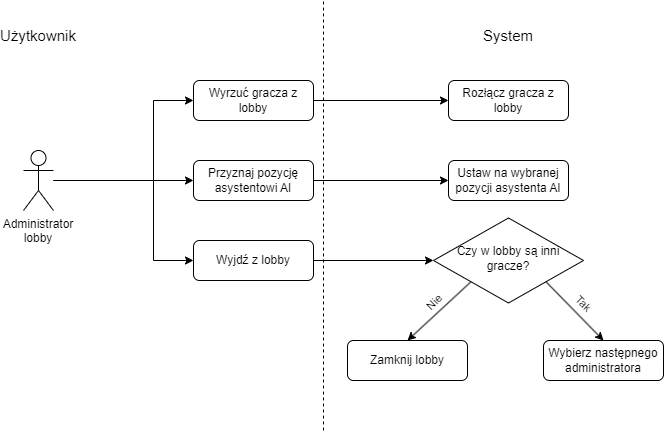
\includegraphics[width=0.9\textwidth]{img/schematy/manage_lobby.png}
  \caption{Schemat zarządzania lobby}
  \label{fig:figma_xd_manage_lobby}
\end{figure}

\FloatBarrier


\subsubsection{Zgłoszenie gotowości}
Użytkownik po dołączeniu do lobby może zgłosić gotowość do rozgrywki poprzez
naciśnięcie przycisku "Ready". Przejście wszystkich użytkowników w~lobby
w~stan gotowości spowoduje rozpoczęcie się gry.


\subsection{Gra w brydża}

\subsubsection{Licytacja}

\begin{figure}[hbt!]
  \centering
  \includegraphics[width=0.9\textwidth]{img/schematy/bid.png}
  \caption{Schemat zgłoszenie odzywki}
  \label{fig:figma_xd_bid}
\end{figure}

Na etapie początkowym gry, uczestnicy mają możliwość zgłaszania odzywek poprzez
aktywację przycisków odpowiadających ich wyborom (Rys.~\ref{fig:figma_xd_bid}).
Mogą licytować kontrakty, pasować lub
deklarować kontrę i~rekontrę. Pierwszy licytujący jest losowo
wybranym graczem. Faza licytacji dobiega końca, gdy odzywka "pas"\xspace zostanie zagrana
trzy razy z rzędu.


\FloatBarrier


\subsubsection{Zagrywanie kart}

Po zakończeniu fazy licytacji gracz może zagrać kartę poprzez
przesunięcie kursora nad kartę i~kliknięcie myszką (Rys.~\ref{fig:figma_xd_play_card}).
Akcja zagrania
będzie dostępna, tylko jeżeli odbędzie się ona w~turze danego gracza
i~wybrana karta może być zagrana.
Dostępność akcji będzie odpowiednio zasygnalizowana w~interfejsie.
Gracz będący partnerem dziadka zagrywa karty w~jego imieniu,
zgodnie z~zasadami gry w~brydża.

\begin{figure}[hbt!]
  \centering
  \includegraphics[width=0.9\textwidth]{img/schematy/play_card.png}
  \caption{Schemat zagrania karty przez użytkownika}
  \label{fig:figma_xd_play_card}
\end{figure}

\FloatBarrier


\subsubsection{Zastąpienie gracza}
W przypadku, gdy jeden z użytkowników opuści grę, jego miejsce zostanie automatycznie
zajęte przez wirtualnego asystenta. Jednakże, jeśli wszyscy użytkownicy
zdecydują się opuścić rozgrywkę, to zostanie ona zakończona.

% \subsection{Obserwowanie rozgrywek}

% Gdy jakaś rozgrywka w~brydża została rozpoczęta i~ma ona status
% publiczny, jest możliwe obejrzenie jej z~panelu \textbf{Watch}.
% Z~listy publicznych rozgrywek należy wybrać interesującą i~kliknąć
% ikonę oka. 
% \end{itemize}

% \begin{figure}[h]
%   \centering
%   \includegraphics[width=\textwidth]{example-image-a}
%   \caption{}
% \end{figure}

% \FloatBarrier


\section{Specyfikacja wymagań funkcjonalnych}

Aplikacja nie tylko powinna być dobrze zaprojektowana i~wygodna
w~użyciu, ale także funkcjonalna. Musi spełniać założone wymagania,
udostępniając odpowiednie funkcjonalności przydatne dla
jej użytkowników. Nie da się jej używać, jeśli brakuje w~niej
wirtualnego asystenta z~odpowiednim
algorytmem AI, czy też elementu
rozgrywki. Bez spełnienia kluczowych wymagań funkcjonalnych,
aplikacja praktycznie nie istnieje. W~tym podrozdziale przedstawiamy
te wymagania.


\subsection{Logowanie i rejestracja nowych użytkowników}
Żeby uzyskać dostęp do funkcjonalności naszej aplikacji, trzeba
posiadać konto i~być zalogowanym. Z~tego względu koniecznością
jest umożliwienie użytkownikom utworzenia konta, logowania się na
nie i~możliwość późniejszego wylogowania. Formularz rejestracji wymaga
podania adresu e-mail, nazwy użytkownika i~hasła. Logowanie odbywa się
poprzez wprowadzenie swojego adresu e-mail i~hasła.


\subsection{Lobby}
W~celu rozegrania partii brydża przeciwko innym graczom
użytkownik musi mieć możliwość utworzenia własnej
rozgrywki oraz dołączenia do istniejącej.

\subsubsection{Utworzenie/Dołączenie do lobby}
Utworzenie, jak i~dołączenie do lobby jest dostępne z~widoku głównego aplikacji. Dołączenie do lobby
odbywa się poprzez wprowadzenie identyfikatora gry. Po utworzeniu lobby użytkownik może
wysłać jego identyfikator innym użytkownikom, zapraszając ich do dołączenia.

\subsubsection{Zarządzanie lobby}
Host powinien mieć możliwość dostosowania lobby według swoich preferencji przed
rozpoczęciem gry. Host ma prawo wyrzucić gracza z~lobby, zmienić jego pozycję lub przekazać
mu swoje uprawnienia. Dodatkowo host powinien móc przydzielić wybrane pozycje
wirtualnym asystentom.


\subsection{Rozpoczęcie rozgrywki}
Kiedy wszystkie miejsca w~lobby zostaną zajęte przez graczy, którzy zgłoszą gotowość do gry,
rozgrywka zostaje rozpoczęta.
Wszyscy użytkownicy zostają przeniesieni do ekranu gry.


\subsection{Rozgrywka}
Głównym celem i~podstawową funkcjonalnością naszej aplikacji jest
rozgrywka w~brydża. Zaczyna się ona od fazy licytacji, po której
gracze wykładają karty zgodnie z~zasadami gry. Gra kończy się po rozegraniu
trzynastu lew. Po skończonej rozgrywce użytkownikowi wyświetlany jest ekran z~wynikami.

\subsection{Wyświetlenie wyników}
Ważne jest, żeby użytkownicy po skończeniu partii mogli zobaczyć
podsumowanie całej rozgrywki. Użytkownikowi wyświetlana jest liczba
zdobytych lew. Dzięki temu użytkownicy mogą na koniec porównać rezultat rozgrywki
ze swoimi założeniami z~fazy licytacji i~lepiej oceniać swoje możliwości w~przyszłych rozgrywkach.


\subsection{Opuszczenie rozgrywki}
Użytkownik może nie tylko wyjść z~lobby, ale także w~dowolnym momencie
opuścić rozgrywkę. W~takim przypadku miejsce użytkownika w~trakcie
rozgrywki zastępuje wirtualny asystent.



% TODO

\section{Specyfikacja wymagań niefunkcjonalnych}
W~naszym projekcie aplikacji do gry w~brydża
istotą jest zapewnienie nie tylko wszystkich potrzebnych wymagań
funkcjonalnych, ale także wygodnej i~intuicyjnej rozgrywki. Niewiele osób
będzie chętnie korzystać z~aplikacji, choćby miała ona rozbudowane
spektrum funkcji, jeśli jej działanie będzie niestabilne i~pozbawione
intuicyjności. W~tym podrozdziale przedstawiamy wymagania
niefunkcjonalne aplikacji, które są równie ważne, jak zdefiniowane
wcześniej wymagania funkcjonalne.


\subsection{Dostępność}
Zdecydowano, aby tworzona aplikacja była dostępna w~formie webowej.
Dzięki temu będzie on dostępny zarówno dla użytkowników
Windows, MacOS, Linux, jak i~innych systemów operacyjnych posiadających
przeglądarkę wspierającą najnowsze standardy.
Kluczowe jest dostosowanie interfejsów tak,
aby były wygodne i~funkcjonalne nawet na urządzeniach o~niewielkich
rozmiarach ekranu, umożliwiając płynne korzystanie z~aplikacji również
na urządzeniach mobilnych.


\subsection{Użyteczność}
Priorytetem aplikacji jest zapewnienie łatwości obsługi
i~zrozumiałości działania elementów interfejsu.
Istotne jest, aby interfejs użytkownika
był intuicyjny, estetyczny i~nie zniechęcał potencjalnych użytkowników
oraz nie utrudniał korzystania z~aplikacji. Ustalono, aby podczas
projektowania interfejsu użytkownika kierować się zasadami
dobrego UI/UX.
Za cel postanowiono stworzenie minimalistycznego i~uporządkowanego
interfejsu, który zapewniłby spójność na wszystkich podstronach aplikacji.
Wykorzystane mają zostać ikony o~jednakowym znaczeniu na wszystkich stronach,
co ułatwi nawigację. Dodatkowo zastosujemy stałą gamę starannie
dobranych kolorów dla elementów interfejsu, co pozwoli nam utrzymać
spójny styl podczas projektowania kolejnych widoków. Aplikacja
będzie oferować tryb jasny i~ciemny, aby użytkownicy mogli z~niej
wygodnie korzystać w~zależności od preferencji lub pory dnia.
Ponadto, wszystkie podstrony będą responsywne, co będzie oznaczać,
że elementy interfejsu będą zachowywać pełną funkcjonalność,
niezależnie od rozmiaru okna przeglądarki, na którym są wyświetlane.

\subsection{Niezawodność}
Wirtualny asystent do gry w~brydża ma być tworzony z~myślą o~nauce
i~doskonaleniu umiejętności, ale także konkurencji i~wzajemnym
rozgrywkom pomiędzy użytkownikami. Konieczne jest więc wprowadzenie logiki
gry z~największą dokładnością. Błędy w~działaniu aplikacji podczas
rozgrywki mogłyby wpłynąć na wynik gry oraz wprowadzić nowych użytkowników
w~zakłopotanie, a~bardziej doświadczonych w~stan irytacji.
Niezwykle istotne jest również uniknięcie sytuacji, w~których
dochodziłoby do utraty połączenia lub braku synchronizacji pomiędzy
użytkownikami. Takie incydenty mogą zrujnować całą rozgrywkę i~zdecydowanie
obniżyć wartość jednej z~kluczowych funkcjonalności aplikacji, jaką
jest możliwość rozgrywania partii między graczami.
Również błędy implementacyjne logiki gry sprawiłyby problemy
z~działaniem asystenta. Nie jest to dopuszczalne, zważając na to,
że asystent ma być konkurencyjnym i~sprawnie działającym rozwiązaniem.

